\documentclass{beamer}

\title{An argumentation based solution to making schedules}
\author{Pim van der Meulen \and Ren\'e Mellema \and Xeryus Stokkel}
\date{October 24, 2016}

\usetheme{Luebeck}

\begin{document}

\frame{\titlepage}

\section{Introduction}
\begin{frame}
	\frametitle{Introduction}
	
\includegraphics[width=0.52\textwidth]{Schedule.jpg}%
	
\includegraphics[width=0.48\textwidth]{Argument.jpg}
\end{frame}

\section{State of the art}
\begin{frame}
	\frametitle{Syllabus Plus}
	\begin{columns}%[c] % the "c" option specifies center vertical alignment
    \column{.8\textwidth} % column designated by a command
    \begin{enumerate}
		\item Used by colleges and universities all over the world, including the University of Groningen
		\item Constraint satisfaction problem solver:
		\begin{enumerate}
			\item Constraints
			\item Rules
			\item Preferences
		\end{enumerate}
	\end{enumerate}
    \column{.2\textwidth}
    
\includegraphics[width=\textwidth]{SyllabusPlus.png}
    \end{columns}	
\end{frame}

\section{Our approach}
\begin{frame}
	\frametitle{Our approach}
\end{frame}

\subsection{Types of arguments to use}
\begin{frame}
	\frametitle{Argument types}
	\begin{enumerate}
		\item Size argument 
		\item Beamer argument
		\item Preference argument
	\end{enumerate}
\end{frame}

\subsection{Ways of making an argument}
\begin{frame}
	\frametitle{Ways of making an argument}
	\begin{enumerate}
		\item Claim
		\item Undercut
		\item Support
	\end{enumerate}
\end{frame}

\subsection{Data input}
\begin{frame}
	\frametitle{Data input}
	\center
	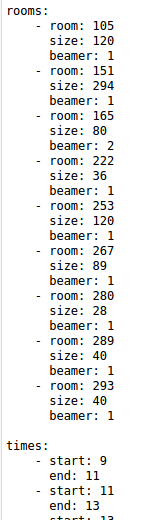
\includegraphics[width=0.2\textwidth]{Rooms.png}%
	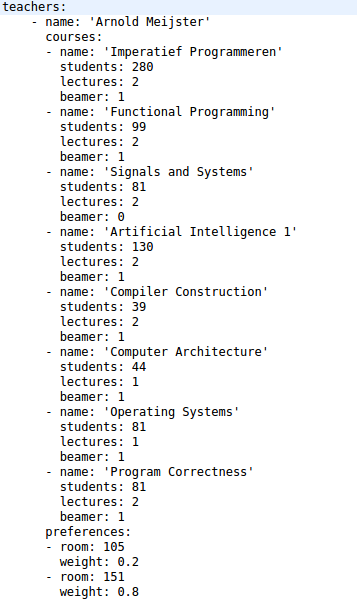
\includegraphics[width=0.365\textwidth]{Teachers.png}
\end{frame}

\section{Results}
\begin{frame}
	\frametitle{Results}
\end{frame}

\section{Relevance}
\begin{frame}
	\frametitle{Relevance}
\end{frame}

\frame{\frametitle{Questions?}}

\end{document}